\section{系统的频率响应}

本节在频域角度,讨论系统如何对输入作用产生输出,介绍系统的频域响应定理与频率响应函数,并给出快速求解系统频率响应函数的方法。

本节要点:
\begin{itemize}
    \item 掌握系统频率响应的概念;
    \item 理解频率响应函数的概念和意义;
    \item 掌握频率响应函数的求解方法。
\end{itemize}

%============================================================
\subsection{频域响应定理与频率响应函数}

\begin{theorem}[系统的频域响应定理]
若一个零状态LTI系统满足绝对稳定的条件,即$\int_{-\infty}^{+\infty}{\left| h\left( t \right) \right|dt}$收敛,则系统对于任意非周期信号$x\left( t \right) $在时域的输出可以表示为卷积:
\[
y\left( t \right) =x\left( t \right) \ast h\left( t \right)
\]
在频域的输出可以表示为傅里叶变换的乘积:
\[
Y\left( \omega \right) =X\left( \omega \right) \cdot H\left( \omega \right)
\]
\begin{itemize}
    \item $x\left( t \right) ,y\left( t \right) $:输入输出信号的时域表达式;
    \item $h\left( t \right) $:系统的冲激响应;
    \item $X\left( \omega \right) ,Y\left( \omega \right) $:输入输出信号的傅里叶变换;
    \item $H\left( \omega \right) $:{\bf 系统的频率响应函数}(frequency response function),或称{\bf 系统函数}(system function),即$h\left( t \right) $的傅里叶变换。
\end{itemize}
\end{theorem}

这表明,一个绝对稳定的LTI系统对任何输入的信号,系统会单独作用其各个频率分量的幅度和相位:
\begin{align*}
&\left| Y\left( \omega \right) \right|=\left| X\left( \omega \right) \right|\cdot \left| H\left( \omega \right) \right| \\
&\angle Y\left( \omega \right) =\angle X\left( \omega \right) +\angle H\left( \omega \right)
\end{align*}
以简单的正弦信号为例,若信号$x\left( t \right) =A\cos \left( \omega _0t+\varphi \right) $,则输出:
\[
y\left( t \right) =A\left| H\left( \omega _0 \right) \right|\cos \left( \omega _0t+\varphi +\angle H\left( \omega _0 \right) \right)
\]
\begin{itemize}
    \item 若系统是无源系统,则$\left| H\left( \omega _0 \right) \right|\leqslant 1$,表示衰减,若系统为有源系统,对应$\left| H\left( \omega _0 \right) \right|>1$,表示放大;
    \item 由于因果性,系统都会将相位往后拉$\angle H\left( \omega _0 \right) $。
\end{itemize}

从定义上来说,$H\left( \omega \right) $是系统的$h\left( t \right) $的傅里叶变换,$h\left( t \right) $是系统对$\delta \left( t \right) $的响应。
由于$\delta \left( t \right) \leftrightarrow 1$,所以从频域上看,$H\left( \omega \right) $是系统对于输入$X\left( \omega \right) =1$的响应。
明白了这一点,也就明白了为什么$H\left( \omega \right) $会被称为“频率响应函数”,指的是系统对各个频率的响应。

%============================================================
\subsection{时域响应和频域响应}

至此,时域响应和频域响应讨论完毕。

在时域我们通过卷积模型描述系统,系统的输出为冲激响应对输入进行卷积运算的结果,不同的系统表现为不同的$h\left( t \right) $。
在频域我们通过傅里叶变换描述系统,输出为频率响应和输入信号的乘积,不同的系统表现为不同的$H\left( \omega \right) $。
无论是卷积模型还是傅里叶变换,本质上都是系统微分方程的反映,是微分方程的冲激函数的解在时域和频域的不同体现。
\[
y\left( t \right) \overset{h\left( t \right) \leftrightarrow H\left( \omega \right)}{=}\begin{cases}
	x\left( t \right) \ast h\left( t \right)\\
	\mathscr{F} ^{-1}\left[ H\left( \omega \right) \cdot X\left( \omega \right) \right]\\
\end{cases}
\]

%============================================================
\subsection{频率响应函数的求解}

\begin{tcolorbox}
系统的频率响应函数可以从定义上求解,但这涉及求解微分方程,特别是高阶的微分方程,几乎无解。
这里给出一个求解的方法。
\end{tcolorbox}

若有限维度LTI系统的微分方程如下:
\[
y^{\left( n \right)}\left( t \right) +\sum_{k=0}^{n-1}{A_ky^{\left( k \right)}\left( t \right)}=\sum_{k=0}^m{B_kx^{\left( k \right)}\left( t \right)}
\]
根据傅里叶变换的导数性质$\frac{d^nx\left( t \right)}{dt^n}\leftrightarrow \left( i\omega \right) ^n\cdot X\left( \omega \right) $,两边取傅里叶变换:
\[
\left( i\omega \right) ^nY\left( \omega \right) +\sum_{k=0}^{n-1}{A_k\left( i\omega \right) ^kY\left( \omega \right)}=\sum_{k=0}^m{B_k\left( i\omega \right) ^kX\left( \omega \right)}
\]
整理后得到:
\[
H\left( \omega \right) =\frac{\sum_{k=0}^m{B_k\left( i\omega \right) ^k}}{\left( i\omega \right) ^n+\sum_{k=0}^{n-1}{A_k\left( i\omega \right) ^k}}
\]

\begin{tcolorbox}
由于$i$代表虚数符号,所以进入到傅里叶章节后用$k$作为连加的序数。
\end{tcolorbox}

%============================================================
\subsection{例}

\begin{example}
如下RC电路,设电压源为输入,电容两端电压为输出,分析系统的频率响应函数。
\begin{figure}[h]
\centering
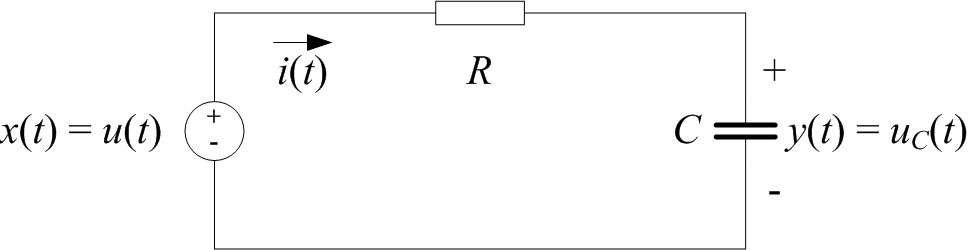
\includegraphics[height=2cm]{1.5.1-1.png}
\end{figure}
\end{example}

根据之前对该电路的分析,系统微分方程有:
\[
\frac{dy}{dt}+\frac{1}{RC}y=\frac{1}{RC}x
\]
直接运用上面的推导结论,有:
\[
H\left( \omega \right) =\frac{\sum_{k=0}^m{B_k\left( i\omega \right) ^k}}{\left( i\omega \right) ^n+\sum_{k=0}^{n-1}{A_k\left( i\omega \right) ^k}}=\frac{\frac{1}{RC}\left( i\omega \right) ^0}{\left( i\omega \right) ^1+\frac{1}{RC}\left( i\omega \right) ^0}=\frac{\frac{1}{RC}}{i\omega +\frac{1}{RC}}
\]
用最原始的方法,求解微分方程->求解冲激响应->获得频率响应函数。
求解微分方程及冲激响应:
\begin{align*}
&y=\frac{1}{RC}e^{-\frac{t}{RC}}\int_0^t{e^{\frac{\tau}{RC}}x\left( \tau \right) d\tau} \\
&h=\left. y \right|_{x=\delta}=\frac{1}{RC}e^{-\frac{t}{RC}}\int_0^t{e^{\frac{\tau}{RC}}\delta \left( \tau \right) d\tau}=\frac{1}{RC}e^{-\frac{t}{RC}}
\end{align*}
求解频率响应函数:
\begin{align*}
&\because e^{-bt}u\left( t \right) \leftrightarrow \frac{1}{b+i\omega} \\
&\therefore H\left( \omega \right) =\frac{1}{RC}\frac{1}{\frac{1}{RC}+i\omega}
\end{align*}

~

\begin{example}
设有弹簧减震装置,系统的微分方程为$x-D\frac{dy}{dt}-Ky=M\frac{d^2y}{dt^2}$,求解其频率响应函数。
\end{example}

先将方程化为:
\[
\frac{d^2y}{dt^2}+\frac{D}{M}\frac{dy}{dt}+\frac{K}{M}y=\frac{1}{M}x
\]
运用本节的方法:
\begin{align*}
H\left( \omega \right) &=\frac{\sum_{k=0}^m{B_k\left( i\omega \right) ^k}}{\left( i\omega \right) ^n+\sum_{k=0}^{n-1}{A_k\left( i\omega \right) ^k}}=\frac{\frac{1}{M}}{\left( i\omega \right) ^2+\left( i\omega \right) \frac{D}{M}+\frac{K}{M}} \\
&=\frac{1}{-M\omega ^2+iD\omega +k}
\end{align*}




